%!TEX root = practicum2.tex
\subsection*{The Intersection of two Line Segments}
	From here on we will define the cross product of two dimension vectors \vec{v} and \vec{w} as following:
	\begin{equation}\label{eq:a:crossproduct}
		\vec{v} \times \vec{w} = - v_2 w_1 + v_1 w_2
	\end{equation}
	where $q_n$ represents the $n$'th element of vector \vec{q}.\\

	In this section we will consider the intersection of the line segments $l_1$ and $l_2$ \cite{so} which are defined as:
	\begin{align}
		l_1 &= \vec{p} + t \vec{r} \label{eq:a:l1}\\
		l_2 &= \vec{q} + u \vec{s} \label{eq:a:l2}.
	\end{align}
	Any point lies on $l_1$ if and only if that point can be expressed as \eqref{eq:a:l1} with $0 \leq t \leq 1$. Using this we can define the intersection \vec{I} of the two line segments as following: the line segments $l_1$ and $l_2$ intersect if we can find values for $t$ and $u$ such that $t, u \in [0, 1]$ and:
		\begin{equation}
			\vec{p} + t \vec{r} = \vec{q} + u \vec{s}
		\end{equation}
	Rewriting this equation gives us expressions for $u$ and $t$:
	\begin{align}
		t &= \frac{\vec{q} - \vec{p} \times \vec{s}}{\vec{r} \times \vec{s}} \label{eq:a:solt}\\
		u &= \frac{\vec{q} - \vec{p} \times \vec{r}}{\vec{r} \times \vec{s}} \label{eq:a:solu}
	\end{align}
	If the denominator, ($\vec{r} \times \vec{s}$), of \eqref{eq:a:solt} or \eqref{eq:a:solu} is zero the lines are parallel, since the cross product of two parallel vectors is zero.

	If we know that we are not dividing by zero we can compute $u$ and $t$ and check if they are in the range $[0,1]$.\\

	This intersection test is implemented in the class \t{LineSegment}, see \autoref{lst:a:linesegment} which is part of the module \t{utilities}. The code to compute \t{r_cross_s}, \t{u_numerator} and \t{t_numerator} was generated with Mathematica, see \autoref{lst:a:lineSegmentIntersectionMat}.\\

	\begin{lstlisting}[float, language=Mathematica, label={lst:a:lineSegmentIntersectionMat}, caption={Mathematica code used to compute the value of \t{r_cross_s}, \t{u_numerator} and \t{t_numerator}.}]
	rExtended = {r000, r001, 0};
	sExtended = {s000, s001, 0};
	qExtended = {q000, q001, 0};
	pExtended = {p000, p001, 0};

	rCrossS = Part[Cross[rExtended, sExtended], 3];
	tNumerator = Part[Cross[(qExtended - pExtended), sExtended], 3];
	uNumerator = Part[Cross[(qExtended - pExtended), rExtended], 3];\end{lstlisting}

	\lstinputlisting[float, firstline=42, lastline=78, label={lst:a:linesegment}, caption={The class \t{LineSegment}. It should be noted that \t{division} has been imported from \t{\_\_future\_\_}.}]{../utilities.py}

\subsection*{Point in a Polygon}
	Since we know that the polygon $P$ is convex we can test quite simply if the point $p$ is inside the polygon by translating the polygon so that $p$ becomes the origin of $P$. The point $p$ is now in the polygon if all angles of the from the origin to the vertices of the polygon are in the range $[0, \pi]$. Since we are only interested in the sign of the angle it suffices to take the outer product as defined in \autoref{eq:a:crossproduct}. If the signs of all these cross products are equal the point $p$ lies inside the polygon $P$. \cite{wolfram} The method \t{point_in_polygon} in the module \t{utilities} uses this method to test if a point lies in a polygon, see \autoref{lst:a:pointInPolygon}.

		\lstinputlisting[firstline=6, lastline=23, label={lst:a:pointInPolygon}, caption={The method \t{point_in_polygon}.}]{../utilities.py}

\subsection*{Point in a Half-Plane}
	To test if a point lies inside a half-plane defined by an edge we have introduced the method \t{vertex_in_half_plane} in the module \t{utilities}, see \autoref{lst:a:vertexInHalfPlane}. This method uses the definition of the half plane given by \citeauthor{o1982new}.

	\lstinputlisting[firstline=26, lastline=39, label={lst:a:vertexInHalfPlane}, caption={The method \t{vertex_in_half_plane}.}]{../utilities.py}

\subsection*{The Algorithm}
	The algorithm presented by \citeauthor{o1982new} finds intersections of the edge $\dot{p}$ and $\dot{q}$ by advancing the edge that points in the direction of the other edge. If neither $\dot{p}$ points at $\dot{q}$ nor $\dot{q}$ points at $\dot{p}$ the outside edge is advanced.  

	\subsubsection*{Implementation}
	The implementation of the algorithm presented by \textcite{o1982new} is implemented in the class \t{ConvexPolygonIntersection}. \t{_algorithm_init} executes all the code before the start of the loop in the algorithm. Each call of \t{_algorithm_step} executes one step of the algorithm. \t{_algorithm_finalize} handles the case where more than $2 \cdot (|P| + |Q|)$ steps have been taken. The code closesly follows the pseudo code presented by \citeauthor{o1982new}.

	\lstinputlisting[float, firstline=106, lastline=109, label={lst:a:polygonIntersectionAlgorithmInit}, caption={The method \t{_algorithm_init} in the class \t{ConvexPolygonIntersection}.}]{../convexPolygonIntersection.py}

	\lstinputlisting[float, firstline=111, lastline=153, label={lst:a:polygonIntersectionAlgorithmStep}, caption={The method \t{_algorithm_step} in the class \t{ConvexPolygonIntersection}.}]{../convexPolygonIntersection.py}

	\lstinputlisting[float, firstline=155, lastline=165x, label={lst:a:polygonIntersectionAlgorithmFinalize}, caption={The method \t{_algorithm_finalize} in the class \t{ConvexPolygonIntersection}.}]{../convexPolygonIntersection.py}

	Since $p_+$, $p_-$, $\dot{p}$, $q_+$, $q_-$, $\dot{q}$ are all derived from $p$ and $q$ I have only stored the index of the current $p$ and $q$ in the variables \t{_p_idx} and \t{_q_idx}. To easily gain access to the derived variables getters and setters have been defined, see \autoref{lst:a:getters}. To increase readability the advancement of the edges has also been implemented as separate methods, see \autoref{lst:a:advance}.

	\lstinputlisting[float, firstline=72, lastline=104, label={lst:a:getters}, caption={The getters in the class \t{ConvexPolygonIntersection}.}]{../convexPolygonIntersection.py}

	\lstinputlisting[float, firstline=60, lastline=70, label={lst:a:advance}, caption={The advancement methods in the class \t{ConvexPolygonIntersection}.}]{../convexPolygonIntersection.py}	

\subsection*{General Implementation}
	To be able to give a step by step visualization of the algorithm \t{ConvexPolygonIntersection} is implemented as an iterator. This allows the user to simply call the method \t{next} on the \t{PolygonIntersection} object. 

	The \t{__init__} method, see \autoref{lst:a:polygonIntersectionInit}, of the iterator initializes the iterator and ensures that number of steps is limited before calling the earlier presented \t{_algorithm_init}. 

	The \t{next} method (\autoref{lst:a:polygonIntersectionNext}) of the iterator increases the step counter and checks if another step is allowed. If allowed it calls \t{_algorithm_step}. If no more steps are allowed \t{_algorithm_finalize} is called before raising a \t{StopIteration} exception. 

	\lstinputlisting[float, firstline=30, lastline=44, label={lst:a:polygonIntersectionInit}, caption={The method \t{__init__} in the class \t{PolygonIntersection}.}]{../convexPolygonIntersection.py}

	\lstinputlisting[float, firstline=50, lastline=57, label={lst:a:polygonIntersectionNext}, caption={The method \t{next} in the class \t{PolygonIntersection}.}]{../convexPolygonIntersection.py}

	The iterator is initiated by calling its constructor with two polygons of which the intersection needs to be computed. Storing the constructed object globally allows us to call \t{next()} in \t{display()} when a certain key is pressed.\\

	To test the algorithm we have used it on two polygons that were, disjoint, two that were intersecting and on a polygon that contained the other polygon see \autoref{fig:a:result}. Changing the initial $q$ to the second to last vertex in the list of vertices representing the polygon yields the intersection in a different order and can change the final $\dot{q}$ and $\dot{p}$, see \autoref{fig:a:result_2}.

	\begin{figure}
		\begin{subfigure}{0.3\textwidth}
			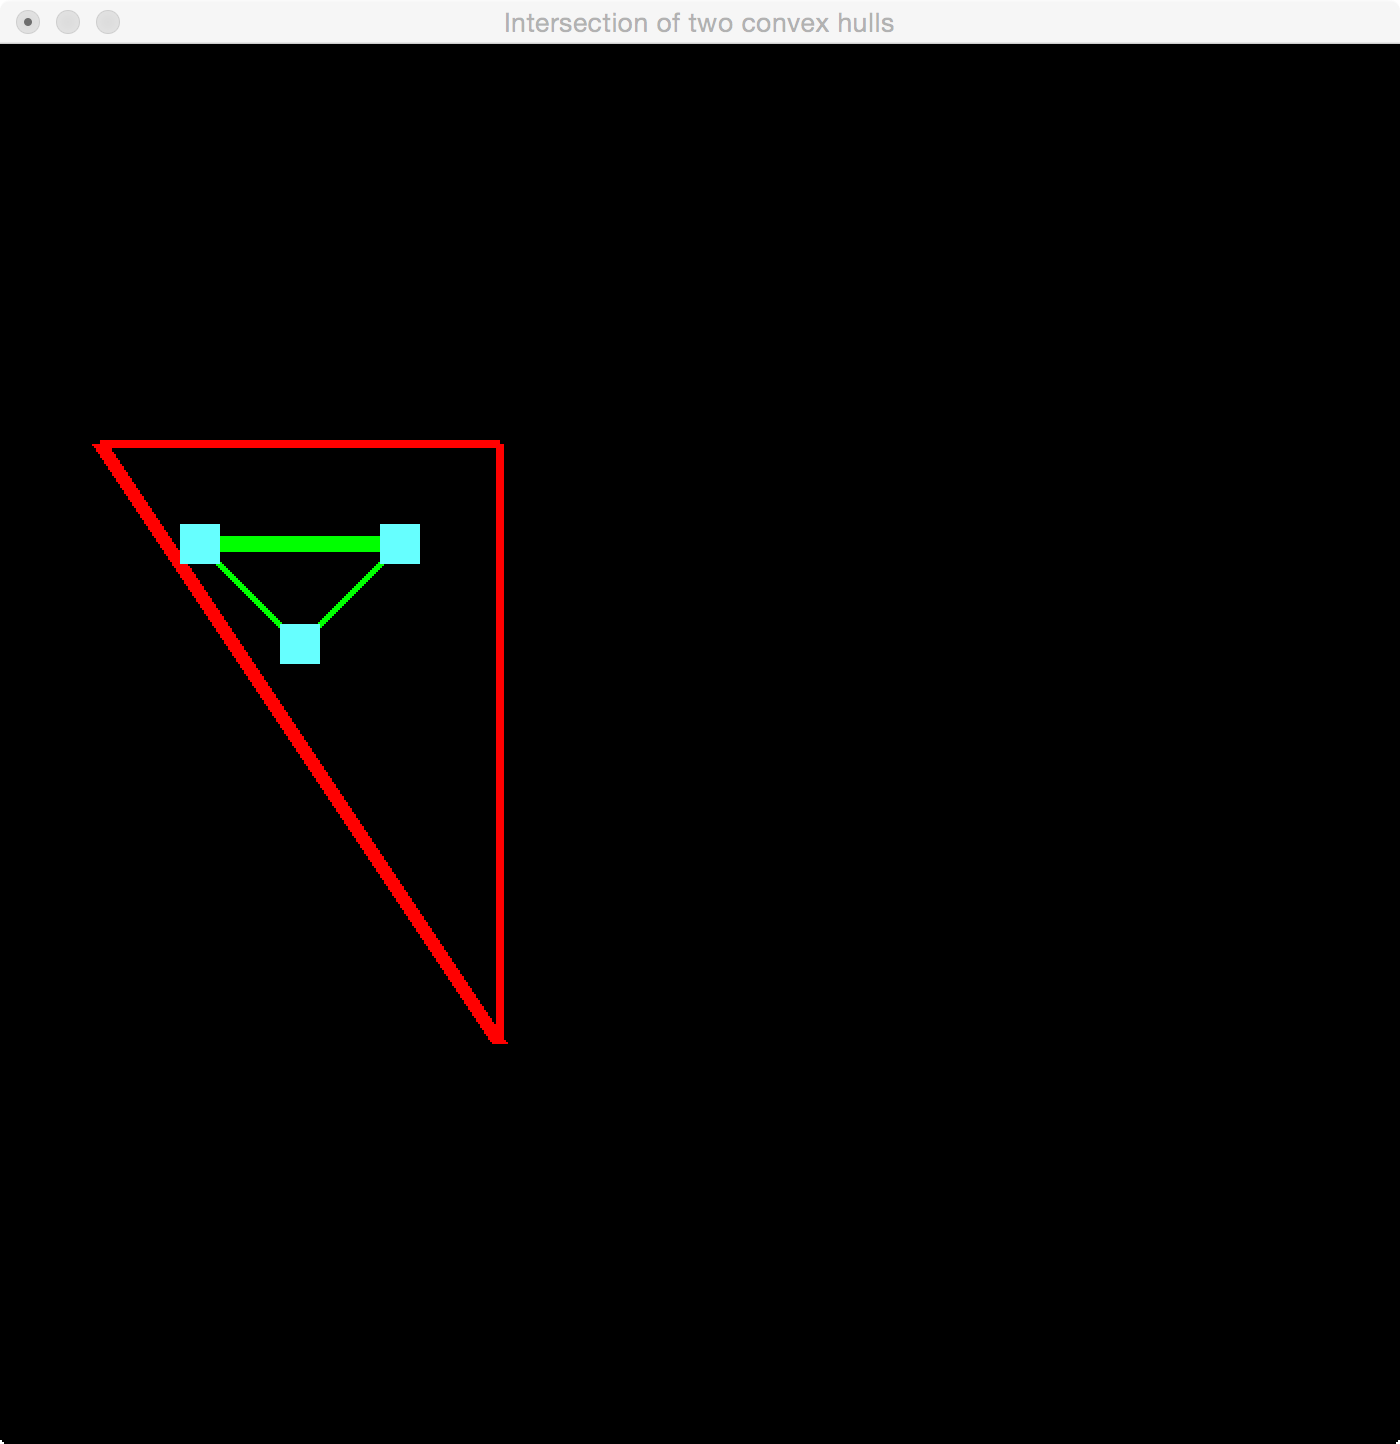
\includegraphics[width=\textwidth]{./img/a_contained}
			\caption{contained}
			\label{subfig:a:results:contained}			
		\end{subfigure}
		\begin{subfigure}{0.3\textwidth}
			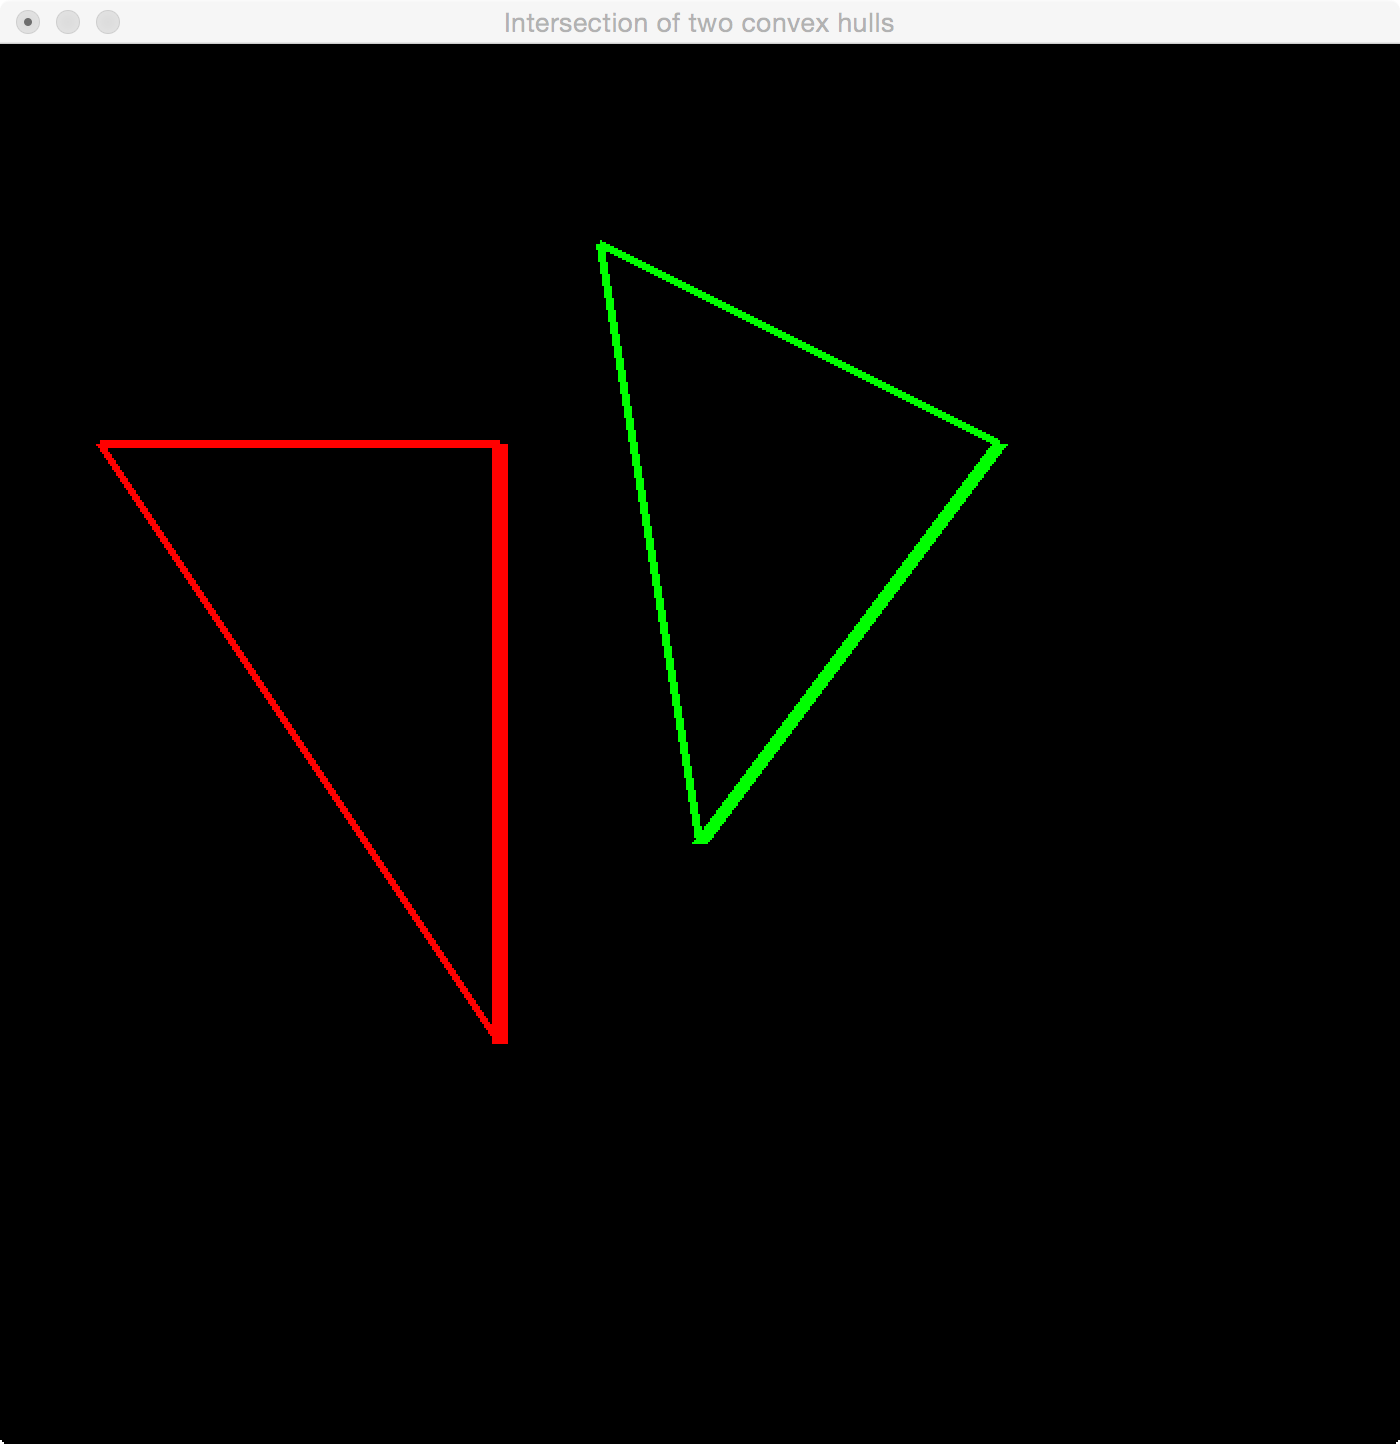
\includegraphics[width=\textwidth]{./img/a_disjoint}
			\caption{disjoint}
			\label{subfig:a:results:disjoint}			
		\end{subfigure}		
		\begin{subfigure}{0.3\textwidth}
			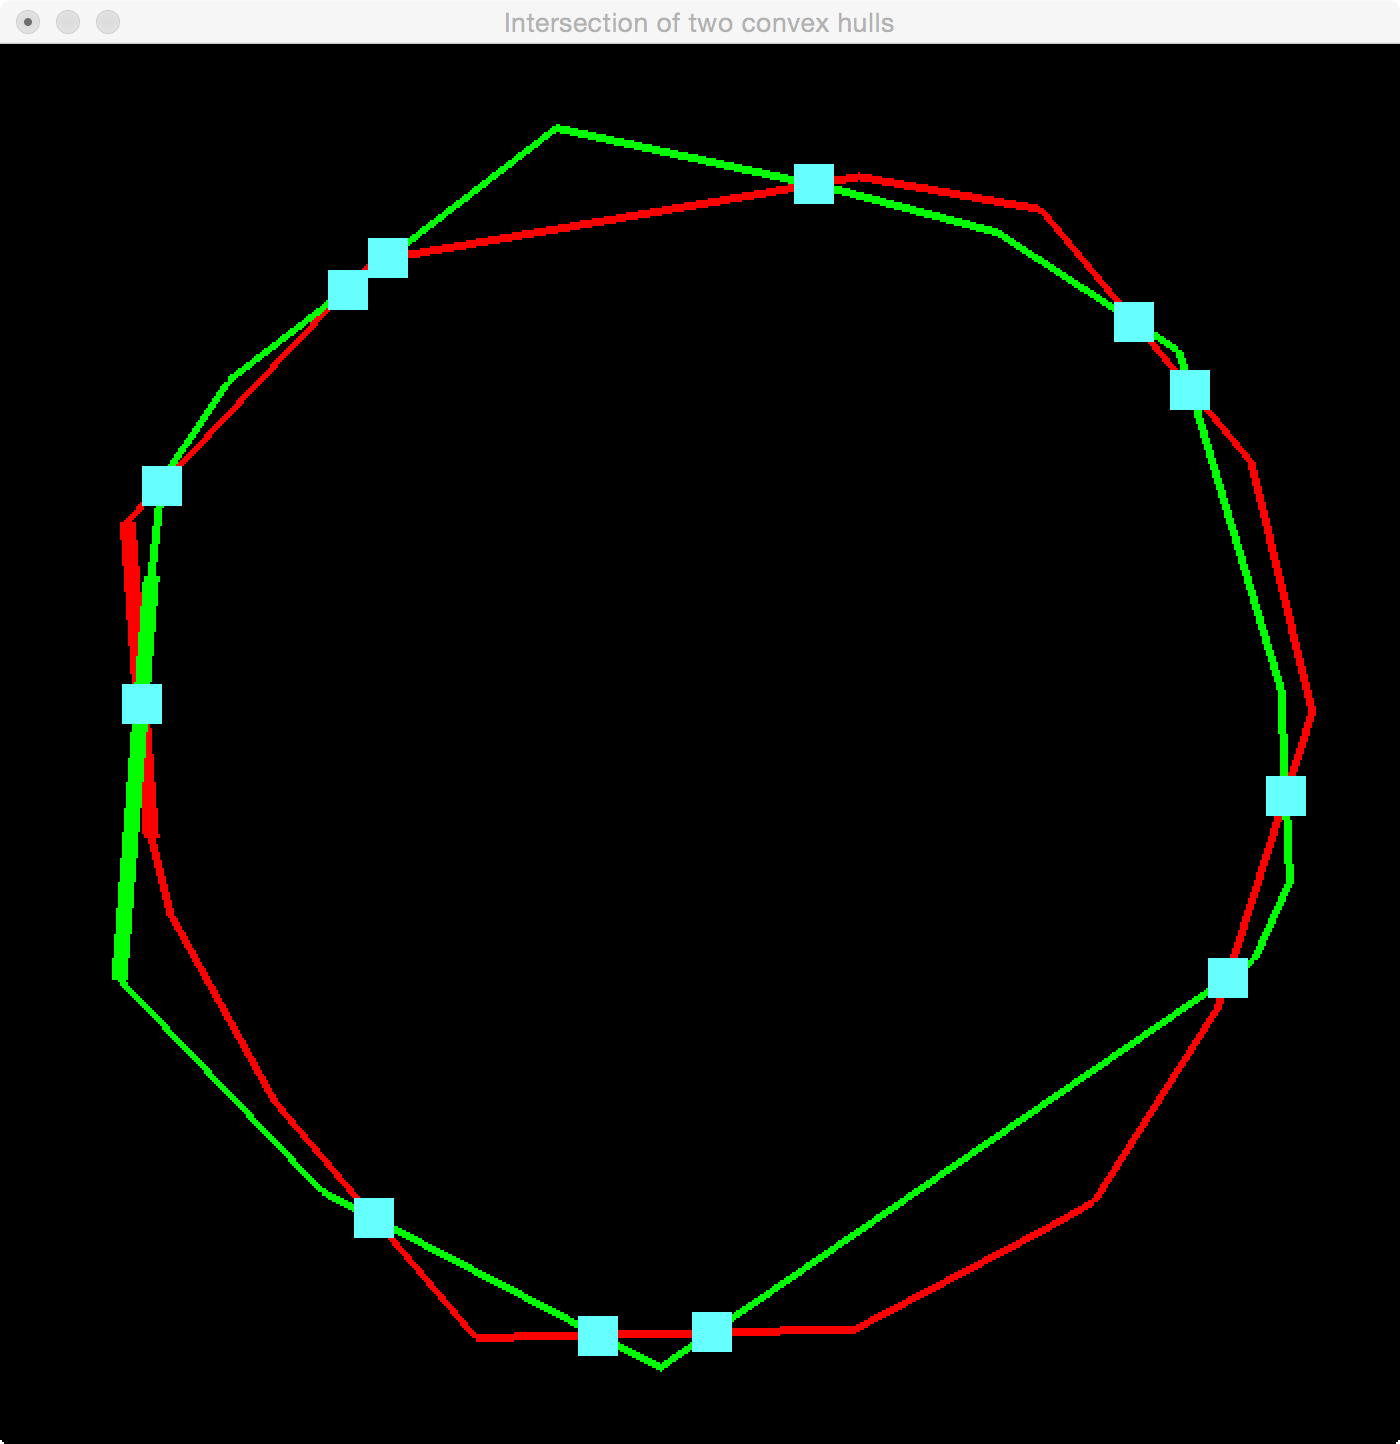
\includegraphics[width=\textwidth]{./img/a_intersecting}
			\caption{intersecting}
			\label{subfig:a:results:intersecting}			
		\end{subfigure}				
		\caption{The final stage of the algorithm for: (\subref{subfig:a:results:contained}) two polygons where one is contained within the other, (\subref{subfig:a:results:disjoint}) two disjoint polygons and (\subref{subfig:a:results:intersecting}) two intersecting polygons. The found intersections points are coloured blue. The thicker edges denote the $\dot{p}$ and $\dot{q}$ at the last step.}
		\label{fig:a:result}
	\end{figure}

	\begin{figure}
		\begin{subfigure}{0.3\textwidth}
			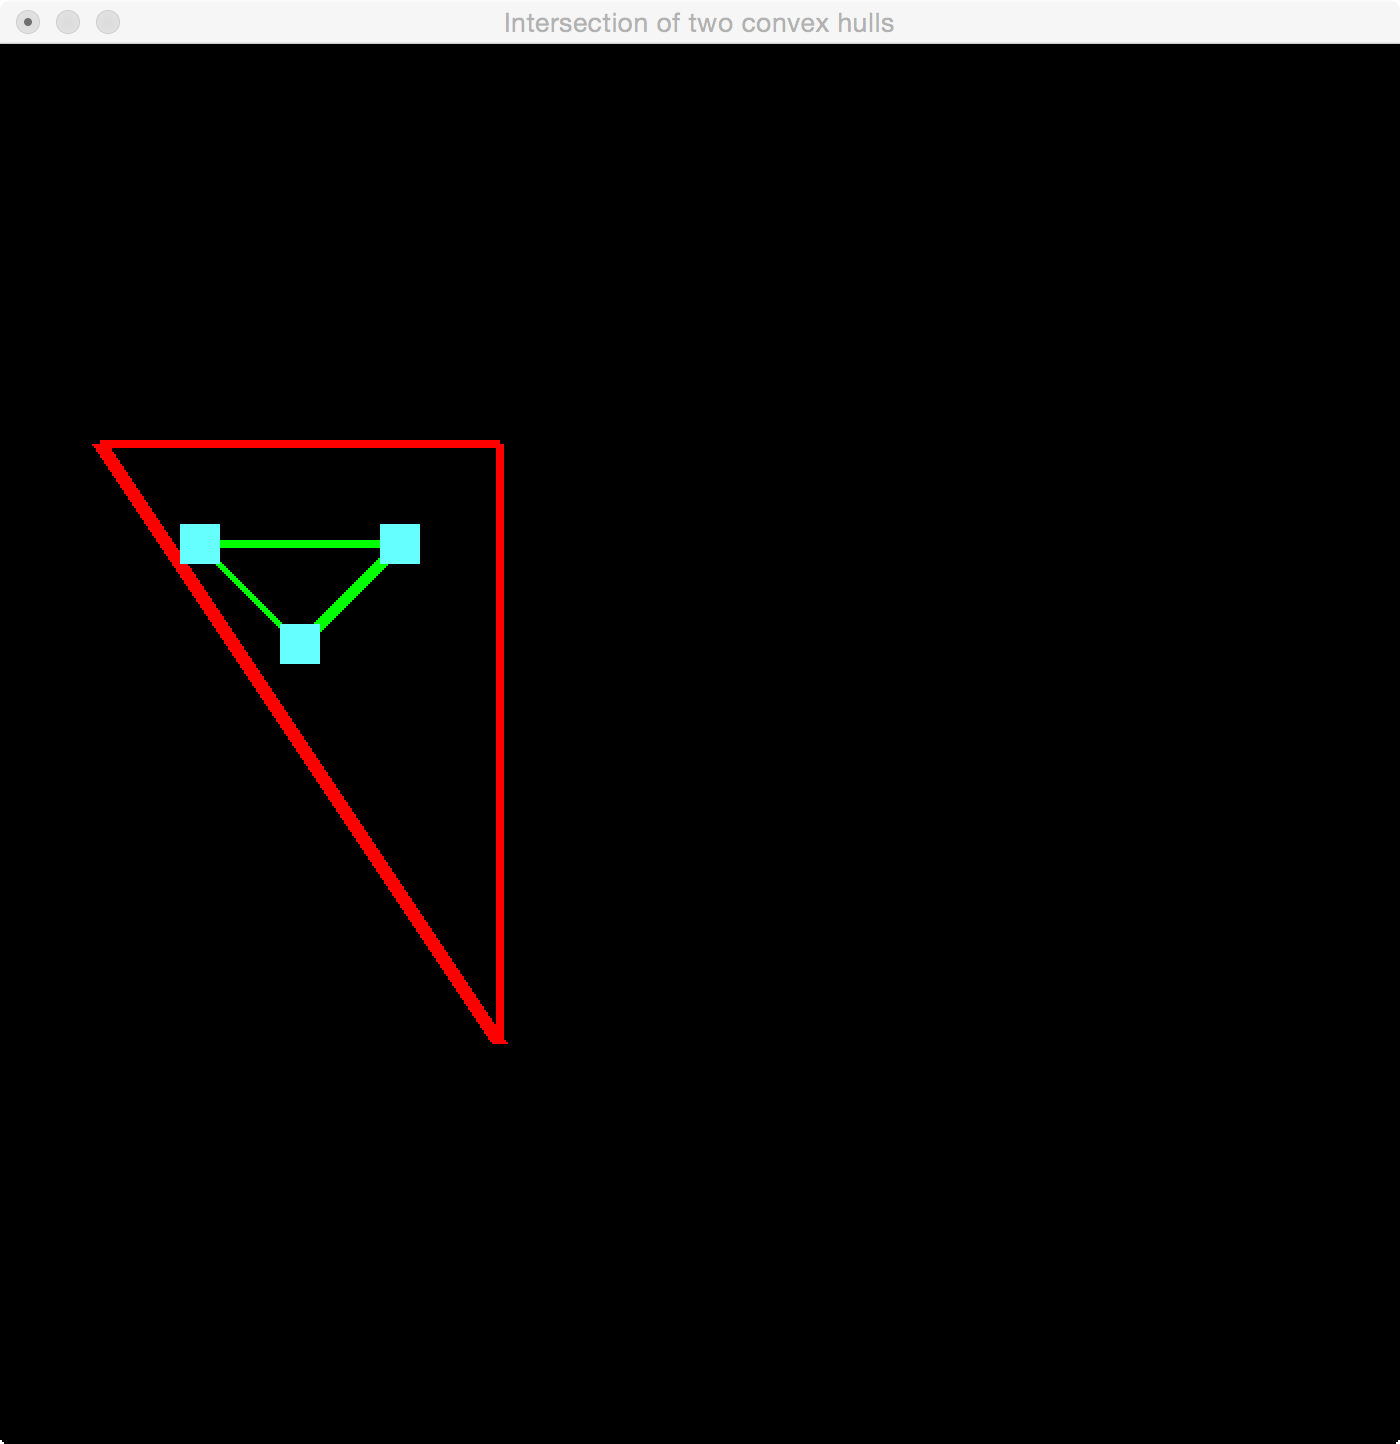
\includegraphics[width=\textwidth]{./img/a_contained_2}
			\caption{contained}
			\label{subfig:a:results:contained_2}			
		\end{subfigure}
		\begin{subfigure}{0.3\textwidth}
			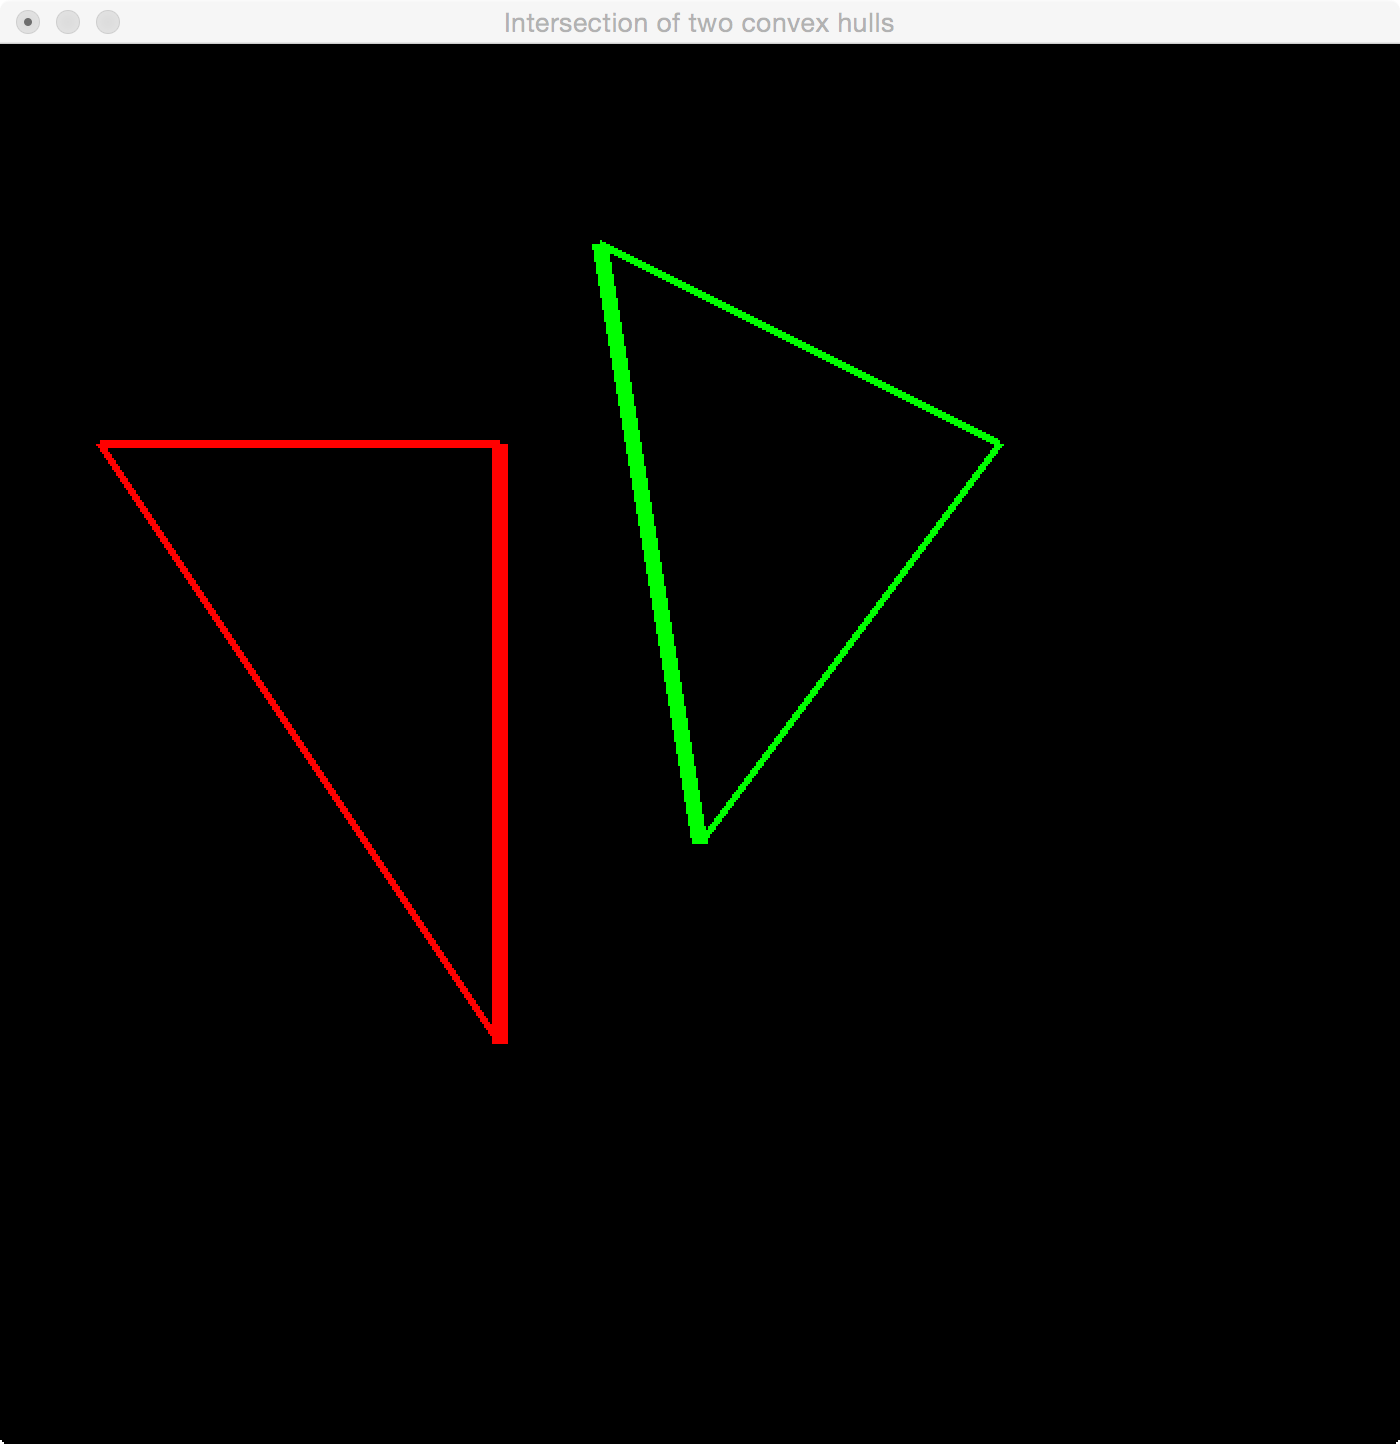
\includegraphics[width=\textwidth]{./img/a_disjoint_2}
			\caption{disjoint}
			\label{subfig:a:results:disjoint_2}			
		\end{subfigure}		
		\begin{subfigure}{0.3\textwidth}
			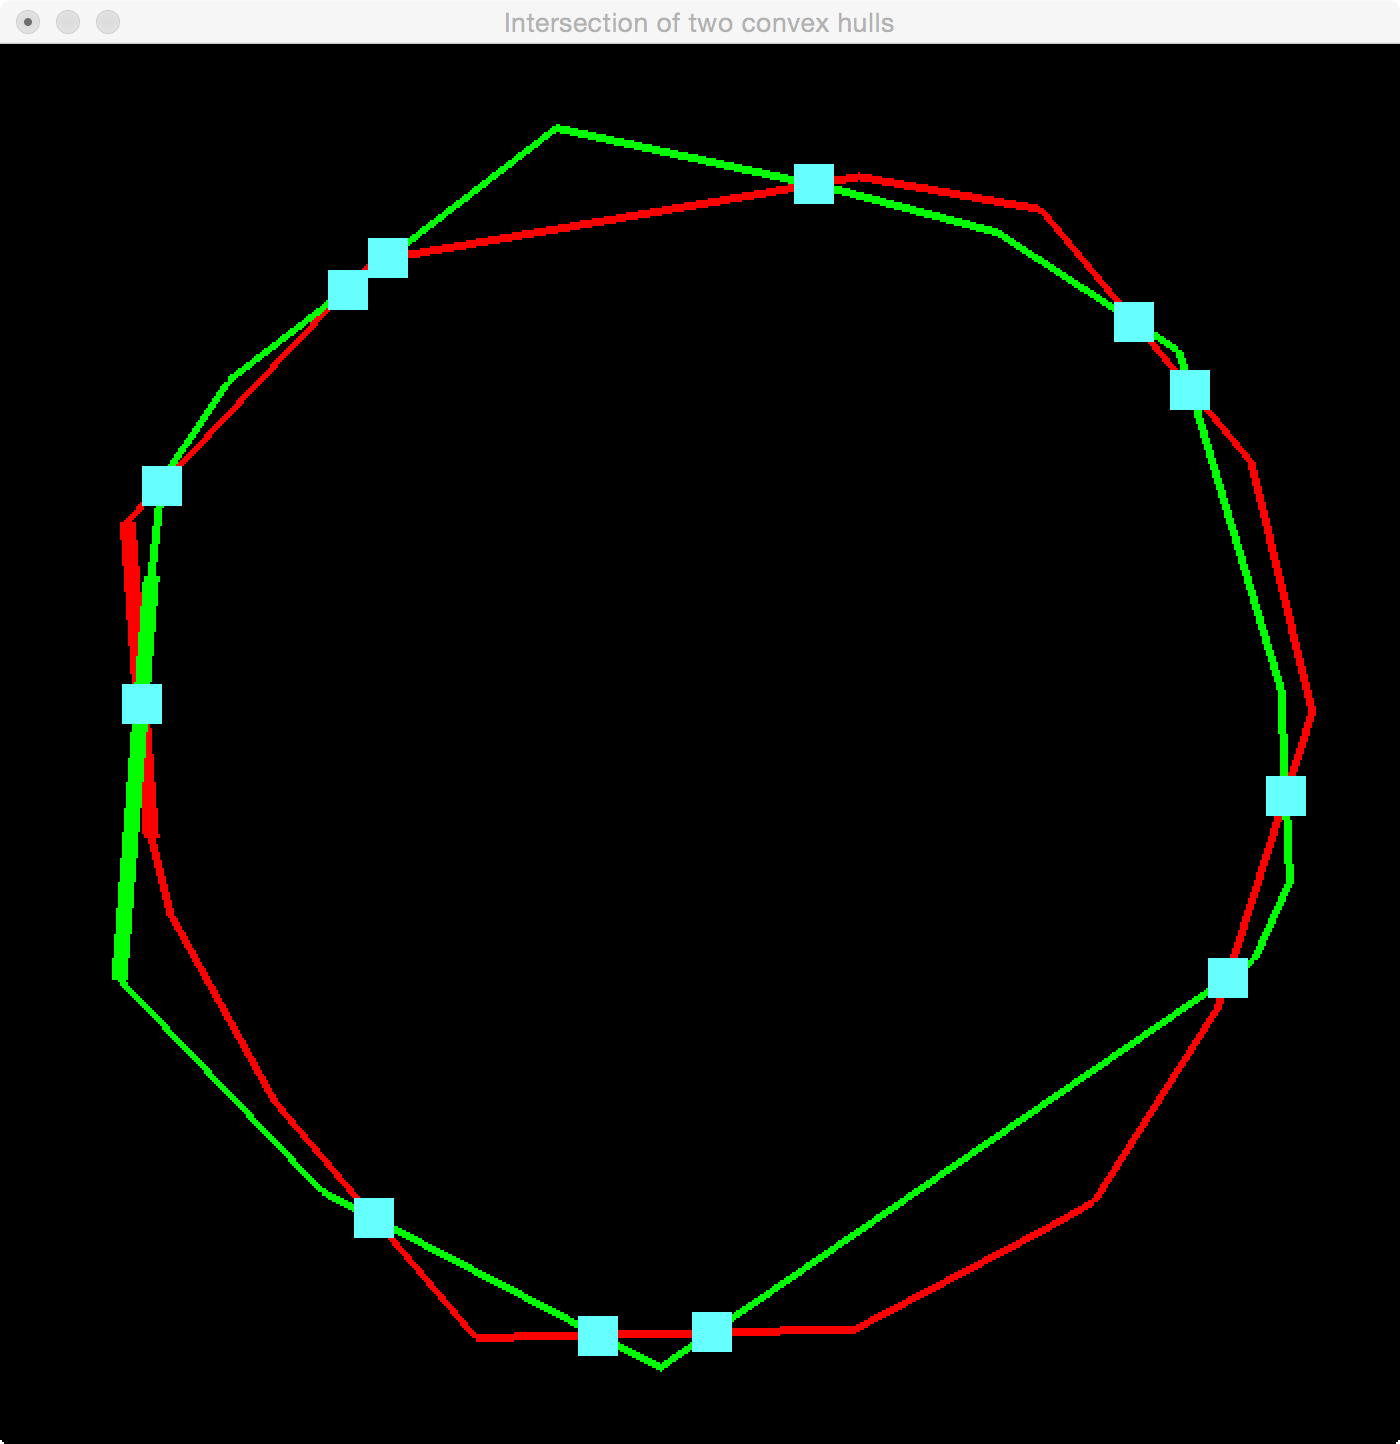
\includegraphics[width=\textwidth]{./img/a_intersecting_2}
			\caption{intersecting}
			\label{subfig:a:results:intersecting_2}			
		\end{subfigure}				
		\caption{The final stage of the algorithm for the same polygons as in \autoref{fig:a:result} but with a different initial $p$ and $q$.}
		\label{fig:a:result_2}
	\end{figure}

	Executing the algorithm on the provided sets \t{P} and \t{Q} results in the following set of intersections:
	[(\num{70.62207492996424}, \num{329.90208847563207}), (\num{80.71128001498256}, \num{220.63611543459012}), (\num{173.66650362806962}, \num{122.63632692888419}), (\num{193.614575574857}, \num{107.2557789542246}), (\num{407.02851445219676}, \num{70.2688269361608}), (\num{567.2108119350485}, \num{138.95033648360118}), (\num{595.2219566014687}, \num{172.61735389897922}), (\num{642.9217273093917}, \num{375.5089532064525}), (\num{613.6005907744503}, \num{467.24741089356974}), (\num{355.7061886957287}, \num{644.2823942804669}), (\num{299.0449678750348}, \num{645.5605985332704}), (\num{187.2554963213314}, \num{587.374506913511})]
